

\documentclass[11pt,fleqn]{book} % Default font size and left-justified equations

%%%%%%%%%%%%%%%%%%%%%%%%%%%%%%%%%%%%%%%%%
% The Legrand Orange Book
% Structural Definitions File
% Version 2.0 (9/2/15)
%
% Original author:
% Mathias Legrand (legrand.mathias@gmail.com) with modifications by:
% Vel (vel@latextemplates.com)
% 
% This file has been downloaded from:
% http://www.LaTeXTemplates.com
%
% License:
% CC BY-NC-SA 3.0 (http://creativecommons.org/licenses/by-nc-sa/3.0/)
%
%%%%%%%%%%%%%%%%%%%%%%%%%%%%%%%%%%%%%%%%%

%----------------------------------------------------------------------------------------
%	VARIOUS REQUIRED PACKAGES AND CONFIGURATIONS
%----------------------------------------------------------------------------------------

\usepackage[top=3cm,bottom=3cm,left=5.5cm,right=3cm,headsep=10pt,letterpaper,asymmetric]{geometry} % Page margins
% Could use 6cm margin on left 

\usepackage{graphicx} % Required for including pictures
\graphicspath{{Pictures/}} % Specifies the directory where pictures are stored

\usepackage{lipsum} % Inserts dummy text

\usepackage{tikz} % Required for drawing custom shapes

\usepackage[english]{babel} % English language/hyphenation

\usepackage{enumitem} % Customize lists
\setlist{noitemsep} % Reduce spacing between bullet points and numbered lists

\usepackage{booktabs} % Required for nicer horizontal rules in tables

\usepackage{xcolor} % Required for specifying colors by name
%\definecolor{rust}{RGB}{243,102,25} % Define the orange color used for highlighting throughout the book
\definecolor{rust}{RGB}{153, 0, 0} % Define alternate red color

\usepackage{pdftexcmds}



%----------------------------------------------------------------------------------------
%	FONTS
%----------------------------------------------------------------------------------------

\usepackage{avant} % Use the Avantgarde font for headings
%\usepackage{times} % Use the Times font for headings
\usepackage{mathptmx} % Use the Adobe Times Roman as the default text font together with math symbols from the Sym­bol, Chancery and Com­puter Modern fonts

\usepackage{microtype} % Slightly tweak font spacing for aesthetics
\usepackage[utf8]{inputenc} % Required for including letters with accents
\usepackage[T1]{fontenc} % Use 8-bit encoding that has 256 glyphs
\usepackage{relsize} % Allow relative font sizing
\renewcommand\RSlargest{100pt} 
%----------------------------------------------------------------------------------------
%	BIBLIOGRAPHY AND INDEX
%----------------------------------------------------------------------------------------

\usepackage[style=alphabetic,citestyle=numeric,sorting=nyt,sortcites=true,autopunct=true,babel=hyphen,hyperref=true,abbreviate=false,backref=true,backend=biber]{biblatex}
\addbibresource{bibliography.bib} % BibTeX bibliography file
\defbibheading{bibempty}{}

\usepackage{calc} % For simpler calculation - used for spacing the index letter headings correctly
\usepackage{makeidx} % Required to make an index
\makeindex % Tells LaTeX to create the files required for indexing

%----------------------------------------------------------------------------------------
%	MAIN TABLE OF CONTENTS
%----------------------------------------------------------------------------------------

\usepackage{titletoc} % Required for manipulating the table of contents

\contentsmargin{0cm} % Removes the default margin

% Part text styling
\titlecontents{part}[0cm]
{\addvspace{20pt}\centering\large\bfseries}
{}
{}
{}

% Chapter text styling
\titlecontents{chapter}[1.25cm] % Indentation
{\addvspace{12pt}\large\sffamily\bfseries} % Spacing and font options for chapters
{\color{rust!60}\contentslabel[\Large\thecontentslabel]{1.25cm}\color{rust}} % Chapter number
{\color{rust}}  
{\color{rust!60}\normalsize\;\titlerule*[.5pc]{.}\;\thecontentspage} % Page number

% Section text styling
\titlecontents{section}[1.25cm] % Indentation
{\addvspace{3pt}\sffamily\bfseries} % Spacing and font options for sections
{\contentslabel[\thecontentslabel]{1.25cm}} % Section number
{}
{\hfill\color{black}\thecontentspage} % Page number
[]

% Subsection text styling
\titlecontents{subsection}[1.25cm] % Indentation
{\addvspace{1pt}\sffamily\small} % Spacing and font options for subsections
{\contentslabel[\thecontentslabel]{1.25cm}} % Subsection number
{}
{\ \titlerule*[.5pc]{.}\;\thecontentspage} % Page number
[]

% List of figures
\titlecontents{figure}[0em]
{\addvspace{-5pt}\sffamily}
{\thecontentslabel\hspace*{1em}}
{}
{\ \titlerule*[.5pc]{.}\;\thecontentspage}
[]

% List of tables
\titlecontents{table}[0em]
{\addvspace{-5pt}\sffamily}
{\thecontentslabel\hspace*{1em}}
{}
{\ \titlerule*[.5pc]{.}\;\thecontentspage}
[]

%----------------------------------------------------------------------------------------
%	MINI TABLE OF CONTENTS IN PART HEADS
%----------------------------------------------------------------------------------------

% Chapter text styling
\titlecontents{lchapter}[0em] % Indenting
{\addvspace{15pt}\large\sffamily\bfseries} % Spacing and font options for chapters
{\color{rust}\contentslabel[\Large\thecontentslabel]{1.25cm}\color{rust}} % Chapter number
{}  
{\color{rust}\normalsize\sffamily\bfseries\;\titlerule*[.5pc]{.}\;\thecontentspage} % Page number

% Section text styling
\titlecontents{lsection}[0em] % Indenting
{\sffamily\small} % Spacing and font options for sections
{\contentslabel[\thecontentslabel]{1.25cm}} % Section number
{}
{}

% Subsection text styling
\titlecontents{lsubsection}[.5em] % Indentation
{\normalfont\footnotesize\sffamily} % Font settings
{}
{}
{}

%----------------------------------------------------------------------------------------
%	PAGE HEADERS
%----------------------------------------------------------------------------------------

\usepackage{fancyhdr} % Required for header and footer configuration

\pagestyle{fancy}
\renewcommand{\chaptermark}[1]{\markboth{\sffamily\normalsize\bfseries\chaptername\ \thechapter.\ #1}{}} % Chapter text font settings
\renewcommand{\sectionmark}[1]{\markright{\sffamily\normalsize\thesection\hspace{5pt}#1}{}} % Section text font settings
\fancyhf{} \fancyhead[LE,RO]{\sffamily\normalsize\thepage} % Font setting for the page number in the header
\fancyhead[LO]{\rightmark} % Print the nearest section name on the left side of odd pages
\fancyhead[RE]{\leftmark} % Print the current chapter name on the right side of even pages
\renewcommand{\headrulewidth}{0.5pt} % Width of the rule under the header
\addtolength{\headheight}{2.5pt} % Increase the spacing around the header slightly
\renewcommand{\footrulewidth}{0pt} % Removes the rule in the footer
\fancypagestyle{plain}{\fancyhead{}\renewcommand{\headrulewidth}{0pt}} % Style for when a plain pagestyle is specified

% Removes the header from odd empty pages at the end of chapters
\makeatletter
\renewcommand{\cleardoublepage}{
\clearpage\ifodd\c@page\else
\hbox{}
\vspace*{\fill}
\thispagestyle{empty}
\newpage
\fi}

%----------------------------------------------------------------------------------------
%	THEOREM STYLES
%----------------------------------------------------------------------------------------

\usepackage{amsmath,amsfonts,amssymb,amsthm} % For math equations, theorems, symbols, etc

\newcommand{\intoo}[2]{\mathopen{]}#1\,;#2\mathclose{[}}
\newcommand{\ud}{\mathop{\mathrm{{}d}}\mathopen{}}
\newcommand{\intff}[2]{\mathopen{[}#1\,;#2\mathclose{]}}
\newtheorem{notation}{Notation}[chapter]

% Boxed/framed environments
\newtheoremstyle{rustnumbox}% % Theorem style name
{0pt}% Space above
{0pt}% Space below
{\normalfont}% % Body font
{}% Indent amount
{\small\bf\sffamily\color{rust}}% % Theorem head font
{\;}% Punctuation after theorem head
{0.25em}% Space after theorem head
{\small\sffamily\color{rust}\thmname{#1}\nobreakspace\thmnumber{\@ifnotempty{#1}{}\@upn{#2}}% Theorem text (e.g. Theorem 2.1)
\thmnote{\nobreakspace\the\thm@notefont\sffamily\bfseries\color{black}---\nobreakspace#3.}} % Optional theorem note
\renewcommand{\qedsymbol}{$\blacksquare$}% Optional qed square

\newtheoremstyle{blacknumex}% Theorem style name
{5pt}% Space above
{5pt}% Space below
{\normalfont}% Body font
{} % Indent amount
{\small\bf\sffamily}% Theorem head font
{\;}% Punctuation after theorem head
{0.25em}% Space after theorem head
{\small\sffamily{\tiny\ensuremath{\blacksquare}}\nobreakspace\thmname{#1}\nobreakspace\thmnumber{\@ifnotempty{#1}{}\@upn{#2}}% Theorem text (e.g. Theorem 2.1)
\thmnote{\nobreakspace\the\thm@notefont\sffamily\bfseries---\nobreakspace#3.}}% Optional theorem note

\newtheoremstyle{blacknumbox} % Theorem style name
{0pt}% Space above
{0pt}% Space below
{\normalfont}% Body font
{}% Indent amount
{\small\bf\sffamily}% Theorem head font
{\;}% Punctuation after theorem head
{0.25em}% Space after theorem head
{\small\sffamily\thmname{#1}\nobreakspace\thmnumber{\@ifnotempty{#1}{}\@upn{#2}}% Theorem text (e.g. Theorem 2.1)
\thmnote{\nobreakspace\the\thm@notefont\sffamily\bfseries---\nobreakspace#3.}}% Optional theorem note

% Non-boxed/non-framed environments
\newtheoremstyle{rustnum}% % Theorem style name
{5pt}% Space above
{5pt}% Space below
{\normalfont}% % Body font
{}% Indent amount
{\small\bf\sffamily\color{rust}}% % Theorem head font
{\;}% Punctuation after theorem head
{0.25em}% Space after theorem head
{\small\sffamily\color{rust}\thmname{#1}\nobreakspace\thmnumber{\@ifnotempty{#1}{}\@upn{#2}}% Theorem text (e.g. Theorem 2.1)
\thmnote{\nobreakspace\the\thm@notefont\sffamily\bfseries\color{black}---\nobreakspace#3.}} % Optional theorem note
\renewcommand{\qedsymbol}{$\blacksquare$}% Optional qed square
\makeatother

% Defines the theorem text style for each type of theorem to one of the three styles above
\newcounter{dummy} 
\numberwithin{dummy}{section}
\theoremstyle{rustnumbox}
\newtheorem{theoremeT}[dummy]{Theorem}
\newtheorem{assignment}{Assignment}[chapter]

\newtheorem{exerciseT}{Exercise}[chapter]
\theoremstyle{blacknumex}
\newtheorem{exampleT}{Example}[chapter]
\theoremstyle{blacknumbox}
\newtheorem{vocabulary}{Vocabulary}[chapter]
\newtheorem{definitionT}{Definition}[section]
\newtheorem{corollaryT}[dummy]{Corollary}
\theoremstyle{rustnum}
\newtheorem{proposition}[dummy]{Proposition}

%----------------------------------------------------------------------------------------
%	DEFINITION OF COLORED BOXES
%----------------------------------------------------------------------------------------

\RequirePackage[framemethod=default]{mdframed} % Required for creating the theorem, definition, exercise and corollary boxes

% Theorem box
\newmdenv[skipabove=7pt,
skipbelow=7pt,
backgroundcolor=black!5,
linecolor=rust,
innerleftmargin=5pt,
innerrightmargin=5pt,
innertopmargin=5pt,
leftmargin=0cm,
rightmargin=0cm,
innerbottommargin=5pt]{tBox}

% Exercise box	  
\newmdenv[skipabove=7pt,
skipbelow=7pt,
rightline=false,
leftline=true,
topline=false,
bottomline=false,
backgroundcolor=rust!10,
linecolor=rust,
innerleftmargin=5pt,
innerrightmargin=5pt,
innertopmargin=5pt,
innerbottommargin=5pt,
leftmargin=0cm,
rightmargin=0cm,
linewidth=4pt]{eBox}	

% Definition box
\newmdenv[skipabove=7pt,
skipbelow=7pt,
rightline=false,
leftline=true,
topline=false,
bottomline=false,
linecolor=rust,
innerleftmargin=5pt,
innerrightmargin=5pt,
innertopmargin=0pt,
leftmargin=0cm,
rightmargin=0cm,
linewidth=4pt,
innerbottommargin=0pt]{dBox}	

% Corollary box
\newmdenv[skipabove=7pt,
skipbelow=7pt,
rightline=false,
leftline=true,
topline=false,
bottomline=false,
linecolor=gray,
backgroundcolor=black!5,
innerleftmargin=5pt,
innerrightmargin=5pt,
innertopmargin=5pt,
leftmargin=0cm,
rightmargin=0cm,
linewidth=4pt,
innerbottommargin=5pt]{cBox}

% Creates an environment for each type of theorem and assigns it a theorem text style from the "Theorem Styles" section above and a colored box from above
\newenvironment{theorem}{\begin{tBox}\begin{theoremeT}}{\end{theoremeT}\end{tBox}}
\newenvironment{exercise}{\begin{eBox}\begin{exerciseT}}{\hfill{\color{rust}\tiny\ensuremath{\blacksquare}}\end{exerciseT}\end{eBox}}				  
\newenvironment{definition}{\begin{dBox}\begin{definitionT}}{\end{definitionT}\end{dBox}}	
\newenvironment{example}{\begin{exampleT}}{\hfill{\tiny\ensuremath{\blacksquare}}\end{exampleT}}		
\newenvironment{corollary}{\begin{cBox}\begin{corollaryT}}{\end{corollaryT}\end{cBox}}	

%----------------------------------------------------------------------------------------
%	WARNING ENVIRONMENT
%----------------------------------------------------------------------------------------

\newenvironment{warning}{\par\vspace{10pt}\small % Vertical white space above the remark and smaller font size
	\begin{list}{}{
			\leftmargin=35pt % Indentation on the left
			\rightmargin=25pt}\item\ignorespaces % Indentation on the right
		\makebox[-2.5pt]{\begin{tikzpicture}[overlay]
			\node[draw=rust!60,line width=1pt,circle,fill=rust!25,font=\sffamily\bfseries,inner sep=2pt,outer sep=0pt] at (-15pt,0pt){\textcolor{rust}{\textbf{!}}};\end{tikzpicture}} 
		\advance\baselineskip -1pt}{\end{list}\vskip5pt} % Tighter line spacing and white space after remark

%----------------------------------------------------------------------------------------
%	REMARK ENVIRONMENT
%----------------------------------------------------------------------------------------

\newenvironment{remark}{\par\vspace{10pt}\small % Vertical white space above the remark and smaller font size
\begin{list}{}{
\leftmargin=35pt % Indentation on the left
\rightmargin=25pt}\item\ignorespaces % Indentation on the right
\makebox[-2.5pt]{\begin{tikzpicture}[overlay]
\node[draw=rust!60,line width=1pt,circle,fill=rust!25,font=\sffamily\bfseries,inner sep=2pt,outer sep=0pt] at (-15pt,0pt){\textcolor{rust}{R}};\end{tikzpicture}} % Orange R in a circle
\advance\baselineskip -1pt}{\end{list}\vskip5pt} % Tighter line spacing and white space after remark

%----------------------------------------------------------------------------------------
%	SECTION NUMBERING IN THE MARGIN
%----------------------------------------------------------------------------------------

\makeatletter

% just bottom line
%\newmdenv[topline=false,leftline=false,rightline=false]{test123}

%\newmdenv[
%rightline=false, leftline=false, topline=false, bottomline=true,
%linecolor=rust, linewidth=4pt
%]{sectionUnderline}

% Adjusts all numbering for sections and subsections
\renewcommand{\@seccntformat}[1]{  
    \ifnum\pdf@strcmp{#1}{section}=\z@ 
    
    %\llap{\colorbox{gray!15}{\makebox[3.25cm][r]{\textcolor{gray}{\textsc{\@nameuse{secTypeName}}\hspace{0.5em}\relsize{1.25}\textcolor{rust}{\csname the#1\endcsname}}}}\hspace{.5em}}
    \llap{
        %\begin{sectionUnderline}
            \makebox[3.25cm][r]{\textcolor{gray}{\textsc{\@nameuse{secTypeName}}\hspace{0.5em}\relsize{1.25}\textcolor{rust}{\csname the#1\endcsname}}}
            \textcolor{rust}{\hspace{-3.25cm}\rule[-.2cm]{3.13cm}{2pt}}
        %\end{sectionUnderline}
        \hspace{.5em}
    }
    \else
    \llap{\textcolor{rust}{\csname the#1\endcsname}\hspace{1em}}%
    \fi 
   % \llap{\textcolor{rust}{\csname the#1\endcsname}\hspace{1em}}
}  % hspace controls spacing of section number to section name    


\newcommand{\setSectionType}[1]{
    \@namedef{secTypeName}{#1}
}
        
\renewcommand{\section}{\@startsection{section}{1}{-8pt}
{-5ex \@plus -1ex \@minus -.2ex}
{2.0ex \@plus.2ex }
{\normalfont\large\sffamily\bfseries}}


\renewcommand{\subsection}{\@startsection {subsection}{2}{-3pt}
{-3ex \@plus -0.1ex \@minus -.4ex}
{0.5ex \@plus.2ex }
{\normalfont\sffamily\bfseries}}
\renewcommand{\subsubsection}{\@startsection {subsubsection}{3}{\z@}
{-2ex \@plus -0.1ex \@minus -.2ex}
{.2ex \@plus.2ex }
{\normalfont\small\sffamily\bfseries}}                        
\renewcommand\paragraph{\@startsection{paragraph}{4}{\z@}
{-2ex \@plus-.2ex \@minus .2ex}
{.1ex}
{\normalfont\small\sffamily\bfseries}}

%----------------------------------------------------------------------------------------
%	PART HEADINGS
%----------------------------------------------------------------------------------------

% numbered part in the table of contents
\newcommand{\@mypartnumtocformat}[2]{%
\setlength\fboxsep{0pt}%
\noindent\colorbox{rust!20}{\strut\parbox[c][.7cm]{\ecart}{\color{rust!70}\Large\sffamily\bfseries\centering#1}}\hskip\esp\colorbox{rust!40}{\strut\parbox[c][.7cm]{\linewidth-\ecart-\esp}{\Large\sffamily\centering#2}}}%
%%%%%%%%%%%%%%%%%%%%%%%%%%%%%%%%%%
% unnumbered part in the table of contents
\newcommand{\@myparttocformat}[1]{%
\setlength\fboxsep{0pt}%
\noindent\colorbox{rust!40}{\strut\parbox[c][.7cm]{\linewidth}{\Large\sffamily\centering#1}}}%
%%%%%%%%%%%%%%%%%%%%%%%%%%%%%%%%%%
\newlength\esp
\setlength\esp{4pt}
\newlength\ecart
\setlength\ecart{1.2cm-\esp}
\newcommand{\thepartimage}{}%
\newcommand{\partimage}[1]{\renewcommand{\thepartimage}{#1}}%
\def\@part[#1]#2{%
\ifnum \c@secnumdepth >-2\relax%
\refstepcounter{part}%
\addcontentsline{toc}{part}{\texorpdfstring{\protect\@mypartnumtocformat{\thepart}{#1}}{\partname~\thepart\ ---\ #1}}
\else%
\addcontentsline{toc}{part}{\texorpdfstring{\protect\@myparttocformat{#1}}{#1}}%
\fi%
\startcontents%
\markboth{}{}%
{\thispagestyle{empty}%
\begin{tikzpicture}[remember picture,overlay]%
\node at (current page.north west){\begin{tikzpicture}[remember picture,overlay]%	
\node[anchor=north] at (4cm,-3.25cm){\color{rust!60}\fontsize{220}{100}\sffamily\bfseries\@Roman\c@part}; 
\node[anchor=south east] at (\paperwidth-1cm,-\paperheight+1cm){\parbox[t][][t]{8.5cm}{
\printcontents{l}{0}{\setcounter{tocdepth}{1}}%
}};
\node[anchor=north east] at (\paperwidth-1.5cm,-3.25cm){\parbox[t][][t]{15cm}{\strut\raggedleft\color{black!40}\fontsize{30}{30}\sffamily\bfseries#2}};
\end{tikzpicture}};
\end{tikzpicture}}%
\@endpart}
\def\@spart#1{%
\startcontents%
\phantomsection
{\thispagestyle{empty}%
\begin{tikzpicture}[remember picture,overlay]%
\node at (current page.north west){\begin{tikzpicture}[remember picture,overlay]%	
\fill[rust!20](0cm,0cm) rectangle (\paperwidth,-\paperheight);
\node[anchor=north east] at (\paperwidth-1.5cm,-3.25cm){\parbox[t][][t]{15cm}{\strut\raggedleft\color{white}\fontsize{30}{30}\sffamily\bfseries#1}};
\end{tikzpicture}};
\end{tikzpicture}}
\addcontentsline{toc}{part}{\texorpdfstring{%
\setlength\fboxsep{0pt}%
\noindent\protect\colorbox{rust!40}{\strut\protect\parbox[c][.7cm]{\linewidth}{\Large\sffamily\protect\centering #1\quad\mbox{}}}}{#1}}%
\@endpart}
\def\@endpart{\vfil\newpage
\if@twoside
\if@openright
\null
\thispagestyle{empty}%
\newpage
\fi
\fi
\if@tempswa
\twocolumn
\fi}

%----------------------------------------------------------------------------------------
%	CHAPTER HEADINGS
%----------------------------------------------------------------------------------------

% A switch to conditionally include a picture, implemented by  Christian Hupfer
\newif\ifusechapterimage
\usechapterimagetrue
\newcommand{\thechapterimage}{}%
\newcommand{\chapterimage}[1]{\ifusechapterimage\renewcommand{\thechapterimage}{#1}\fi}%
\def\@makechapterhead#1{%
{\parindent \z@ \raggedright \normalfont
\ifnum \c@secnumdepth >\m@ne
\if@mainmatter
\begin{tikzpicture}[remember picture,overlay]
\node at (current page.north west)
{\begin{tikzpicture}[remember picture,overlay]
\node[anchor=north west,inner sep=0pt] at (0,0) {\ifusechapterimage\includegraphics[width=\paperwidth]{\thechapterimage}\fi};
%\draw[anchor=west] (\Gm@lmargin,-9cm) node [line width=2pt,rounded corners=15pt,draw=rust,fill=white,fill opacity=0.5,inner sep=15pt]{\strut\makebox[22cm]{}};

%%%%% Chapter text sizing
%\draw[anchor=west] (\Gm@lmargin-1.3cm,-4cm) node [line width=2pt,rounded corners=15pt,draw=rust,fill=white,fill opacity=0.75,inner sep=15pt]{\strut\makebox[22cm]{}};

%\draw[anchor=west] (\Gm@lmargin-1cm,-4.1cm) node {\huge\sffamily\bfseries\color{black}\thechapter. #1\strut};

% Use larger chapter number

\draw[anchor=west] (\Gm@lmargin-1.3cm,-3.9cm) node [line width=2pt,rounded corners=8pt,draw=rust,fill=white,fill opacity=0.75,inner sep=15pt]{\strut\makebox[22cm]{}};

\draw[anchor=west] (\Gm@lmargin-1cm,-4.0cm) node {\huge\sffamily\bfseries\color{black}{\relsize{2}\thechapter. }#1\strut};


\end{tikzpicture}};
\end{tikzpicture}
\else
\begin{tikzpicture}[remember picture,overlay]
\node at (current page.north west)
{\begin{tikzpicture}[remember picture,overlay]
\node[anchor=north west,inner sep=0pt] at (0,0) {\ifusechapterimage\includegraphics[width=\paperwidth]{\thechapterimage}\fi};
%\draw[anchor=west] (\Gm@lmargin,-9cm) node [line width=2pt,rounded corners=15pt,draw=rust,fill=white,fill opacity=0.5,inner sep=15pt]{\strut\makebox[22cm]{}};

\draw[anchor=west] (\Gm@lmargin,-4cm) node [line width=2pt,rounded corners=15pt,draw=rust,fill=white,fill opacity=0.75,inner sep=15pt]{\strut\makebox[22cm]{}};

\draw[anchor=west] (\Gm@lmargin+.3cm,-4cm) node {\huge\sffamily\bfseries\color{black}#1\strut};
\end{tikzpicture}};
\end{tikzpicture}
%\fi\fi\par\vspace*{270\p@}}}

\fi\fi\par\vspace*{150\p@}}}

%-------------------------------------------

\def\@makeschapterhead#1{%
\begin{tikzpicture}[remember picture,overlay]
\node at (current page.north west)
{\begin{tikzpicture}[remember picture,overlay]
\node[anchor=north west,inner sep=0pt] at (0,0) {\ifusechapterimage\includegraphics[width=\paperwidth]{\thechapterimage}\fi};
\draw[anchor=west] (\Gm@lmargin,-9cm) node [line width=2pt,rounded corners=15pt,draw=rust,fill=white,fill opacity=0.5,inner sep=15pt]{\strut\makebox[22cm]{}};
\draw[anchor=west] (\Gm@lmargin+.3cm,-9cm) node {\huge\sffamily\bfseries\color{black}#1\strut};
\end{tikzpicture}};
\end{tikzpicture}
\par\vspace*{270\p@}}
\makeatother

%----------------------------------------------------------------------------------------
%	HYPERLINKS IN THE DOCUMENTS
%----------------------------------------------------------------------------------------

\usepackage{hyperref}
\hypersetup{hidelinks,backref=true,pagebackref=true,hyperindex=true,colorlinks=false,breaklinks=true,urlcolor= rust,bookmarks=true,bookmarksopen=false,pdftitle={Lab Manual},pdfauthor={Brent Mellor}}
\usepackage{bookmark}
\bookmarksetup{
open,
numbered,
addtohook={%
\ifnum\bookmarkget{level}=0 % chapter
\bookmarksetup{bold}%
\fi
\ifnum\bookmarkget{level}=-1 % part
\bookmarksetup{color=rust,bold}%
\fi
}
}
 % Insert the commands.tex file which contains the majority of the structure behind the template
\usepackage{float}

\usepackage{listings} 
\lstset
{ 
    language=C,
    basicstyle=\ttfamily,
    columns=fullflexible,
    keepspaces=true,
    numbers=none,
    stepnumber=1,
    showstringspaces=false,
    tabsize=1,
    breaklines=true,
    breakatwhitespace=false,
    keywordstyle=\color{blue!80!black},
    stringstyle=\color{red!80!black},
    commentstyle=\color{green!40!black},
    morecomment=[l][\color{magenta!80!black}]{\#}
}

\usepackage{caption}
\captionsetup[figure]{font=small,skip=10pt}

%\usepackage{enumitem}
%\setlist{noitemsep} % or \setlist{noitemsep} to leave space around whole list


%%%%% May be too harsh to prevent paragraph breaks across pages! 
%\interlinepenalty 10000
\widowpenalties 1 10000
\raggedbottom


\newcommand{\ilcode}[1]{
    %\vspace{0.5pt}
    \smallskip
    \colorbox{gray!20!white}{
        \centering
        \parbox{\linewidth-2\fboxsep}{
            \lstinline@#1@
        }
    }
    %\vspace{0.5pt}
}

\newcommand{\code}[3]{
    \begin{figure}[]
        \colorbox{gray!20!white}{
            \parbox{\linewidth-2\fboxsep} {
                \centering 
                \lstinputlisting[language=C]{#1}
            }
        }
        \caption{#2}
        \label{#3}
    \end{figure}
}

\usepackage{textcomp}
\usepackage{wrapfig}
\usepackage{float}

\usepackage{silence} % http://ctan.org/pkg/silence
\ErrorFilter{textcomp}{Symbol \textrightarrow not provided}

% Disable paragraph indentation globally since template was indenting some and not others. (looked terrible)
\setlength{\parindent}{0pt}


%%%%%%%%%%%%%%%%%%%%%%%%%%%%%%%%%%%%%%%%%%%%%%%%%%%%%%%%%%%%%%%%%%%%%%%%%%%%%%%%%%%%%%%%%%%%%%%%%
%%%%                                                                                         %%%%
%%%%       Chapter 5: Embedded Communications and the USART                                  %%%%
%%%%                                                                                         %%%%
%%%%%%%%%%%%%%%%%%%%%%%%%%%%%%%%%%%%%%%%%%%%%%%%%%%%%%%%%%%%%%%%%%%%%%%%%%%%%%%%%%%%%%%%%%%%%%%%%

\setcounter{chapter}{4} % Manually adjust chapter counter to number before desired chapter heading

\begin{document}
	
\chapterimage{chapter_head_2.png} % Chapter heading image
\chapter{Embedded Communications and the USART}

\section{Communication Between Systems}
All computing systems regardless of their size and power, are essentially useless if they don't have some way to communicate with the outside world. Even a large supercomputers are unable to perform any meaningful work without some method of introducing new data into the systems, and another to output a result. 

Naturally this applies to embedded systems as well. In fact the majority of embedded peripherals as well as these labs are directed at either capturing or sending information in and out of the system. In the first lab we introduced the GPIO as the most basic method of data transfer. In the second we used the EXTI controller to allow efficient hardware monitoring of GPIO inputs. The third lab used the capture/compare units in a timer peripheral to generate pseudo-analog signals through PWM. 

This lab introduces the fundamentals of data transfer through digital communication interfaces. These interfaces exist because information is only useful when it can be understood, therefore there must be defined ways of transmitting and interpreting it.

\subsection{Parallel vs Serial}

There are two main schemes, parallel and serial, for moving binary information across electrical connections. These two schemes are opposites of each other and are demonstrated in figure \ref{parallel_serial}. 

\subsubsection{Parallel}
Parallel interfaces transmit entire blocks of data using multiple wires, with each wire representing the state of a single binary bit. In a parallel system the transmitter sets the logical state of each wire, and the receiver samples all of the connections at a single instant. Parallel interfaces have a \textit{bit-width} which represents how many wires are in the connection, and indicates how many bits are sent at one time. Common bit-widths are powers of 2 to make converting into bytes simple. 

\subsubsection{Serial}
Serial interfaces use a single wire, and stream a block of data over time by lining up the bits behind each other. In order to properly transmit data, both the transmitter and receiver must agree on the time duration between data bits, known as the interface's \textit{bit/data rate}. A serial transmitter produces periodic transitions on the single data line corresponding to the data to be sent. The receiver samples this data line on a similar period and appends the sampled value to the end of the received data. 

\begin{figure}[]
    \centering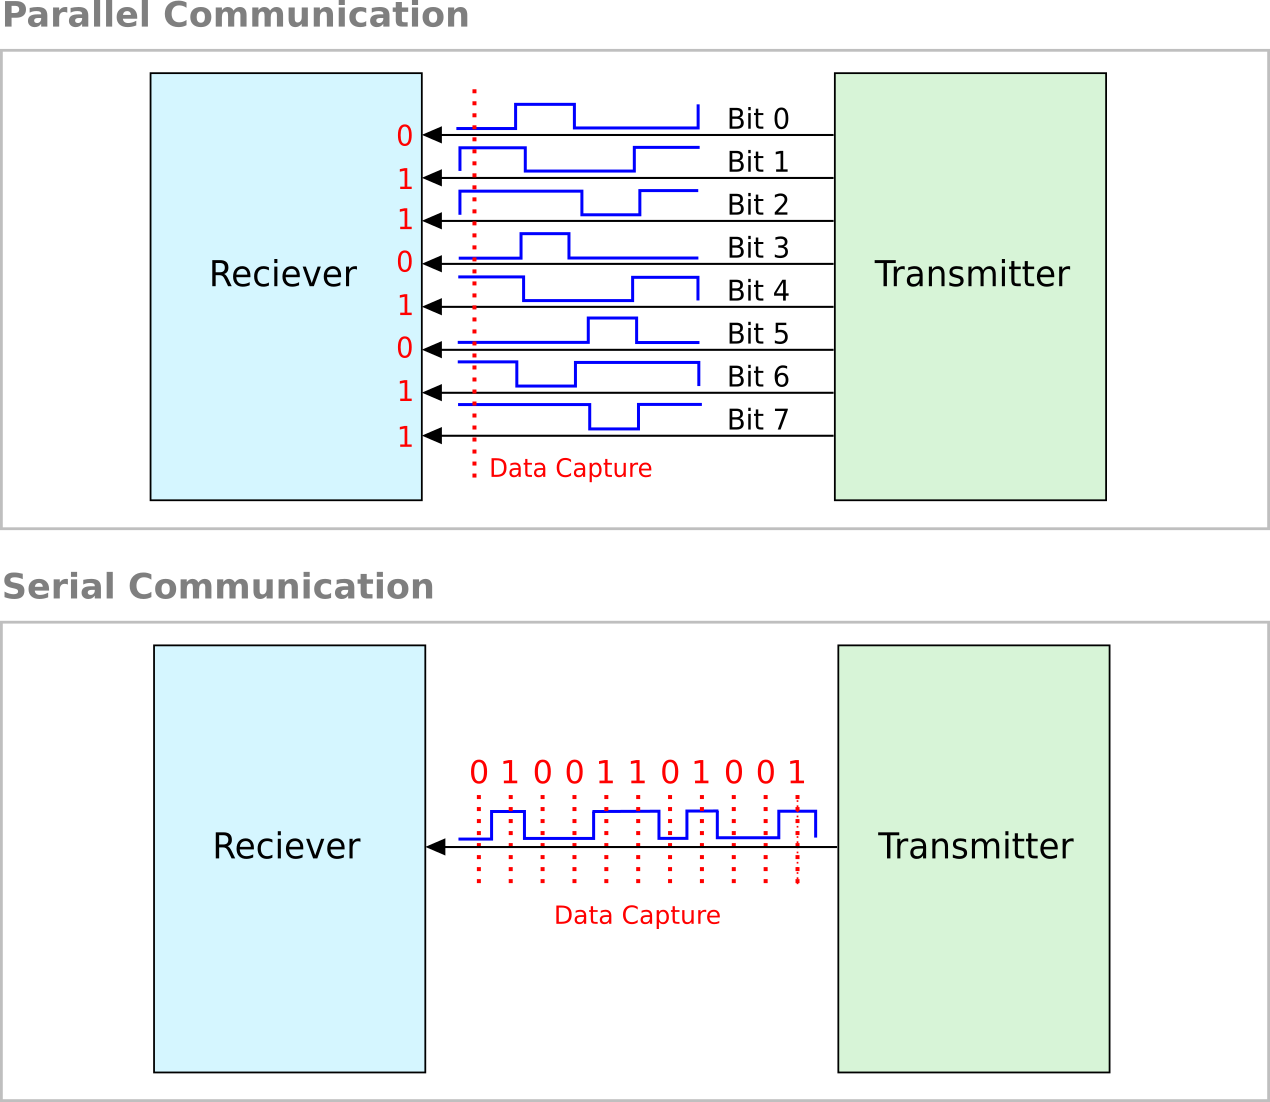
\includegraphics[width=\textwidth]{parallel_serial}
    \caption{Comparison of parallel and serial communication.}
    \label{parallel_serial}
\end{figure}

\subsubsection{Interface Bandwidth and Limitations}
Because parallel connections move entire groups of bits at a time they have a much higher \textit{bandwidth} (throughput) than an equivalent serial connection. Some examples of high-speed parallel connections are the STM32F0's internal device busses (AHB and APB) which connect the ARM processor core to the SRAM, flash memory and other peripherals.

However, despite that equivalent-speed parallel connections have a higher bandwidth, most high-speed device interfaces such as SATA, USB and Ethernet are actually serial interconnects. The reason for this is because parallel connections are far more difficult to design and operate as the distance between the receiver and transmitter increases. With the incredibly high-speeds of today's communications, unless every wire in a connection is exactly the same length it is possible to have some bits arrive after the others. This means that unless the sampling rate of the receiver is slow enough to account for every bit in the connection, incorrect data will be captured.

Serial connections inherently don't have issues with wire-delay. Because bits are streamed one after another, any delays along the wire have a constant effect on the data and can't cause corruption. This enables serial connections to have a much higher bit rate than parallel, and possibly even a higher total bandwidth.

\subsection{Synchronous vs Asynchronous}

Regardless of whether an interface is serial or parallel, there must be be a mechanism that synchronizes when the transmitter and receiver updates or samples the connection. Similar to parallel and serial there are two methods, synchronous and asynchronous, of performing this task. These are demonstrated in figure \ref{synchronous_asynchronous}.

\subsubsection{Synchronous} 
Synchronous systems use a separate ``clock'' signal which notifies the receiver when to sample.  Often the data capture is synchronized to a transition such as rising or falling-edge. Synchronous systems are often simpler in design but require the extra clock connection.

\subsubsection{Asynchronous}
Asynchronous systems operate without a physical clock signal. Some methods of asynchronous communication encode a virtual clock within the transitions of the data while others estimate the time intervals that data should be expected to arrive. Because of the lack of a clock signal, asynchronous interconnects are typically more complex and have lower data rates than synchronous ones. 

\begin{figure}[]
    \centering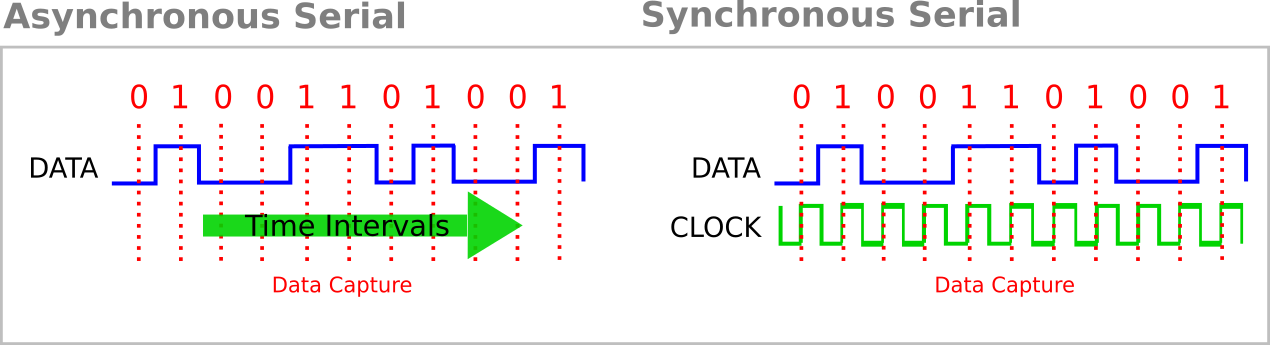
\includegraphics[width=\textwidth]{synchronous_asynchronous}
    \caption{Comparison of synchronous and asynchronous serial communication.}
    \label{synchronous_asynchronous}
\end{figure}

\subsection{Connection Topologies} 
The topology of a communication interface is how the different devices (nodes) and the connections between them are arranged. Some interfaces are strictly point-to-point, which means that they connect only two devices with direct wires. Other interfaces have topologies which allow networks of devices to be connected together. Figure \ref{topologies} demonstrates a few simple topologies. 

\begin{itemize}
    \item \textbf{Daisy-Chain} -- Nodes in a daisy-chained network connect only to their adjacent neighbors. Some are designed to allow data to be passed along to its destination. 
    \item \textbf{Bus/Multi-Drop} -- All nodes on a bus share the same communication lines. This means that only a single device can be transmitting at a time, but all can receive
    \item \textbf{Star} -- All peripheral nodes communicate with a central master node.
    \item \textbf{Mesh} -- Nodes in a mesh network have arbitrary connections to each other. Some mesh networks are hierarchically ordered, others may be fully-connected.   
\end{itemize}



\begin{figure}[]
    \centering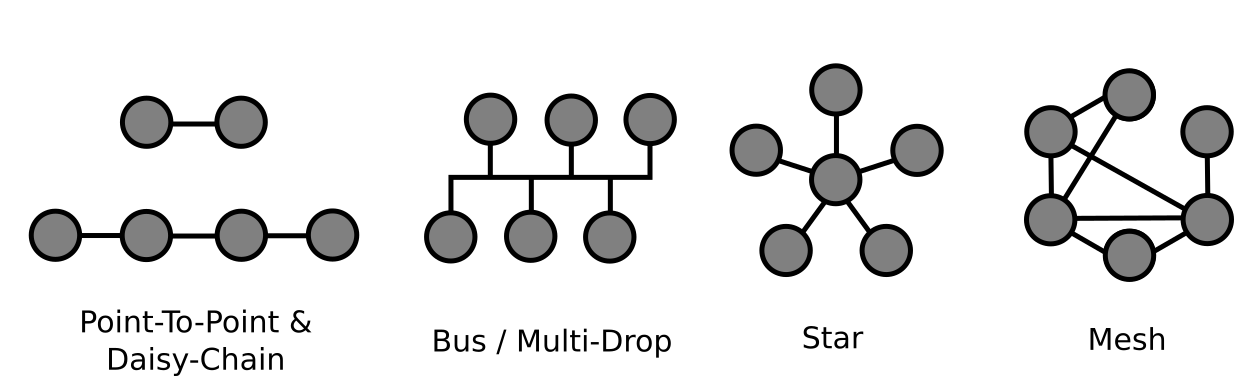
\includegraphics[width=\textwidth]{topologies}
    \caption{Simple network topologies.}
    \label{topologies}
\end{figure}

\section{Communication Standards \& Protocols}

Aside from knowing how to connect and when to sample the inputs, communicating devices must know how to interpret signals into bits and how the patterns of bits make up data. To manage this, all interfaces are combinations of hardware standards and communication protocols. 

\subsection{Hardware Standards}	
Hardware standards define the physical and signaling characteristics of an interface.
A standard typically indicates the medium that the signals are transferred over such as conductive wires, optical, radio frequency or others. The standard defines the method that signals are interpreted into bits. This may be as simple as thresholding a voltage on a wire (single-ended), monitoring the voltage difference or current flow between a pair of wires (differential) or even a modulated waveform. 

Standards often indicate whether an interface is parallel or serial.

\subsection{Communication Protocols}
Hardware standards make it possible to convert an input signal into a collection of bits. However, protocols define the meaning of bits such that they create useful data. 

\subsubsection{Hardware Protocols}
Low level or hardware protocols define how bits are organized to form raw data. This primarily involves the rate that data is sampled and whether the interface has an explicit clock signal or is asynchronous.
Depending on the complexity of the interface, hardware protocols usually include higher-level features such as start/stop signals, error-correction, control flow, message acknowledgment, addressing, data packets and more.

\subsubsection{Software Protocols}	
At this point the communication peripheral's job is complete. Raw data can be converted into a communication signal and back on the receiving end. The last task is to interpret the raw data into useful instructions or information for the user's application.

A software protocol is a device driver that gives meaning to the binary data flowing into and out of the system. These drivers can be as simple as recognizing certain values as commands, or as complex as defining the organization of variable-length data packets.  In order to communicate, the user's application must define a software protocol. 

\subsection{Separating Interface and Protocol}
   
Some communication interfaces have clearly defined separations between the different standards, protocols, and application layers within them. 

For example, IEEE 802.3 is the base standard for wired Ethernet and contains subclasses for the different speeds and modifications that have been made over the years. Built upon these standards are low-level protocols such as MAC, LLC, and PPP. On these is built IP, and IP is the the base of UDP and TCP which are used for raw data connections on conventional computer networks. 

An example of a common software protocol used by computer networks is HTML. This format is used to move website data across the Internet, giving the browser application a known way to interpret raw data into something meaningful. 

Unfortunately, unlike Ethernet, many low-level interfaces such as those used in embedded systems are much more unclear where the boundaries are. Many of these interfaces have protocols and standards that were designed specifically for each other and are called by the same name. 
Because of this, many documents use the terms standard and protocol interchangeably. 

\section{Common Embedded Interfaces}
The STM32F072 has a generous selection of interface peripherals. These can be seen on the first page summary of the chip datasheet. These interfaces differ widely in operation, complexity, and features; however, they all are serial. 

The three most common serial communication interfaces used in embedded systems are TTL RS-232 (TTL-Serial/UART), Serial Peripheral Interface (SPI), and Inter-Integrated Circuit Bus (I2C). 

This lab teaches the basics of TTL RS-232 in the next few sections. SPI and I2C will be covered in later labs, a brief introduction is included here. 

\begin{itemize}
    \item \textbf{Serial Peripheral Interface (SPI)}
    \begin{itemize}
        \item SPI is a synchronous interface typically used for high-speed connections between microcontrollers and external memories or other fast-data devices.
        \item It is a full-duplex interface, which means that both sides transmit and receive at the same time.
    \end{itemize}
    \item \textbf{Inter-Integrated Circuit Bus (I2C)}
    \begin{itemize}
        \item I2C is a low(er) speed synchronous interface designed to allow multiple master devices to share the same set of signal wires. 
        \item It was primarily designed for low-speed sensors, but newer standards have increased the speed where it is also used for other purposes.
    \end{itemize}
\end{itemize}


\section{Introducing RS-232}
\subsection{Conventional RS-232}
Historical use as "serial"
Origin, uses, old connector, voltage levels
\begin{figure}[]
    \centering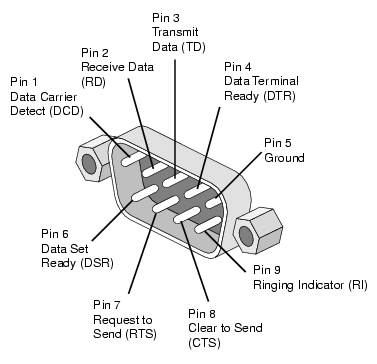
\includegraphics[width=0.3\textwidth]{db9_pinout}
    \caption{Conventional DB9 serial connector and pinout.}
    \label{db9_pinout}
\end{figure} 
\subsection{Embedded TTL RS-232 (TTL-Serial)}
Embedded system use
differences to conventional RS-232
TTL RS-232 Standard Details 
\begin{figure}[]
    \centering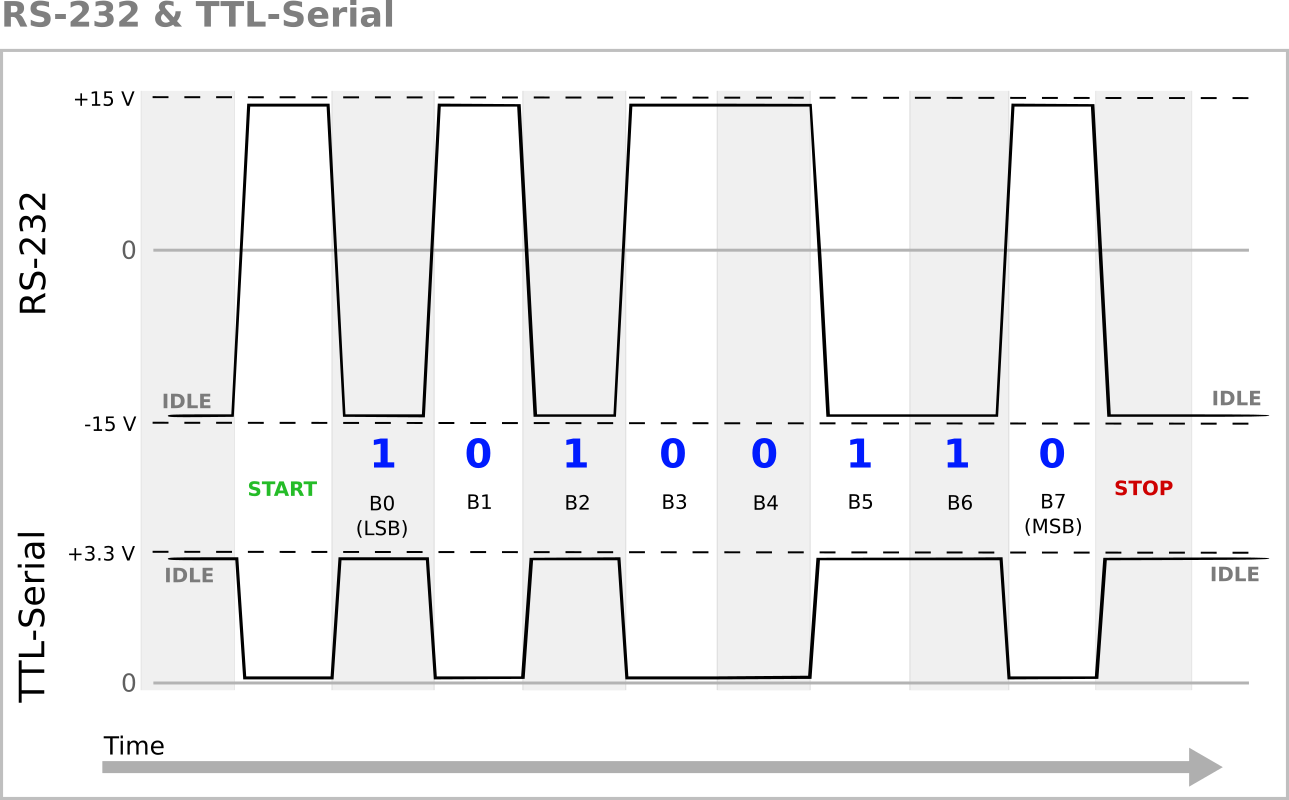
\includegraphics[width=\textwidth]{serial_detail}
    \caption{RS-232 and TTL-Serial logic levels and polarity.}
    \label{serial_detail}
\end{figure}
BAUD rates and Oversampling
Start and Stop Bits
Parity 
USB-UART Cables
Purpose and use, specifically mentioned in later section

\subsection{ASCII Text Encoding}
Old standard for text exchange based on 8-bit characters
Has 128 characters in 7-bits, the last bit is used for parity
Some characters have system meanings such as a newline char
others are non-printing
Some system chars no longer have much meaning in modern systems
Was extended to use all 8-bits 
The original ASCII has since been expanded into the Unicode character standard
Many different encodings for unicode such as UTF8
Will be using base ASCII for embedded communication	
\begin{figure}[]
    \centering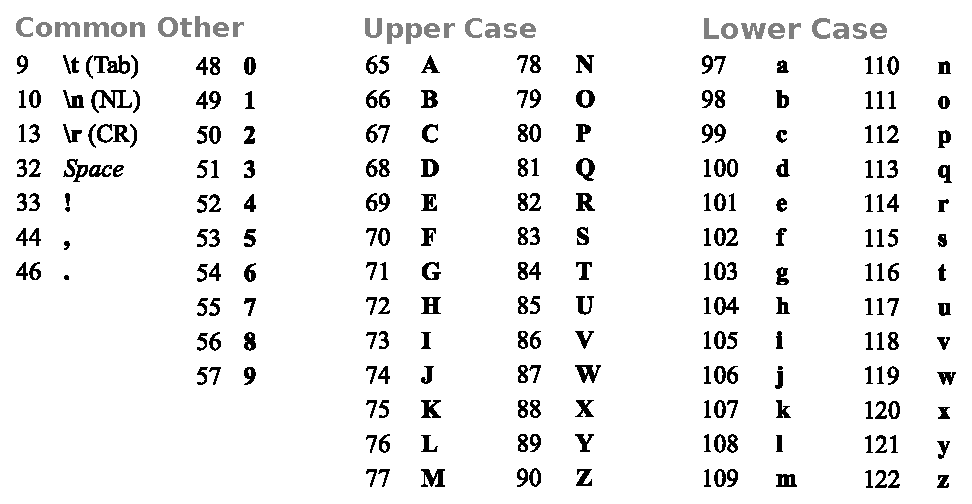
\includegraphics[width=\textwidth]{ascii_table}
    \caption{Subset of the ASCII text encoding standard.}
    \label{ascii_table}
\end{figure}

\section{Introducing the USART}
What the USART is and why it has its name
Typically used for TTL RS-232
Modes of operation
mainly to mention that it has other modes, but we won't discuss them 
\subsection{USART Registers}	
Overview of all registers used for RS-232
Give short description and what each register does (what settings it manages)
Mention other registers and indicate that they won't need them
\subsection{Configuring the BAUD Rate}	
Configuring the BAUD rate registers
Basic equations of calculating baud rate
How to load into the mantissa and fractional baud registers
\subsection{Blocking vs Non-blocking Operation}
mainly mention that you can use buffers and interrupts to make code that doesn't wait around until transmission is complete. 
mention why it's bad to wait sometimes
won't be doing non-blocking drivers in this lab (later lab perhaps?)
\begin{figure}[]
    \centering
\includegraphics[width=\textwidth]{blocking_nonblocking}
    \caption{Blocking and non-blocking drivers.}
    \label{blocking_nonblocking}
\end{figure}
\subsection{Performing Basic Transmits and Receives}
Give flowcharts for blocking receive and transmit
\begin{figure}[]
    \centering
\includegraphics[width=\textwidth]{blocking_flowchart}
    \caption{Flowchart for simple RX/TX communications on the USART.}
    \label{blocking_flowchart}
\end{figure}
Explicitly say when they need to wait/check a flag for this condition before moving onward. 
Don't give actual bit names, but they should be able to use the register descriptions to know where to look
Give pretty obvious hints as to what they should look for when searching for bits.
\subsubsection{Text Formatting}
No printf yet... need to build own string transmit, string compare and eventually numeric value to ASCII character functions
Kiel provides a miniature version of the c standard library called microlib
Can configure and use printf with our USART, but won't in this lab. (later labs?)

\section{Using a USB-UART Cable and the Terminal}
\subsection{The USB-UART Cable}
Using the USB-USART cable and Putty Terminal program
Using and connecting the cable

\begin{figure}[]
    \centering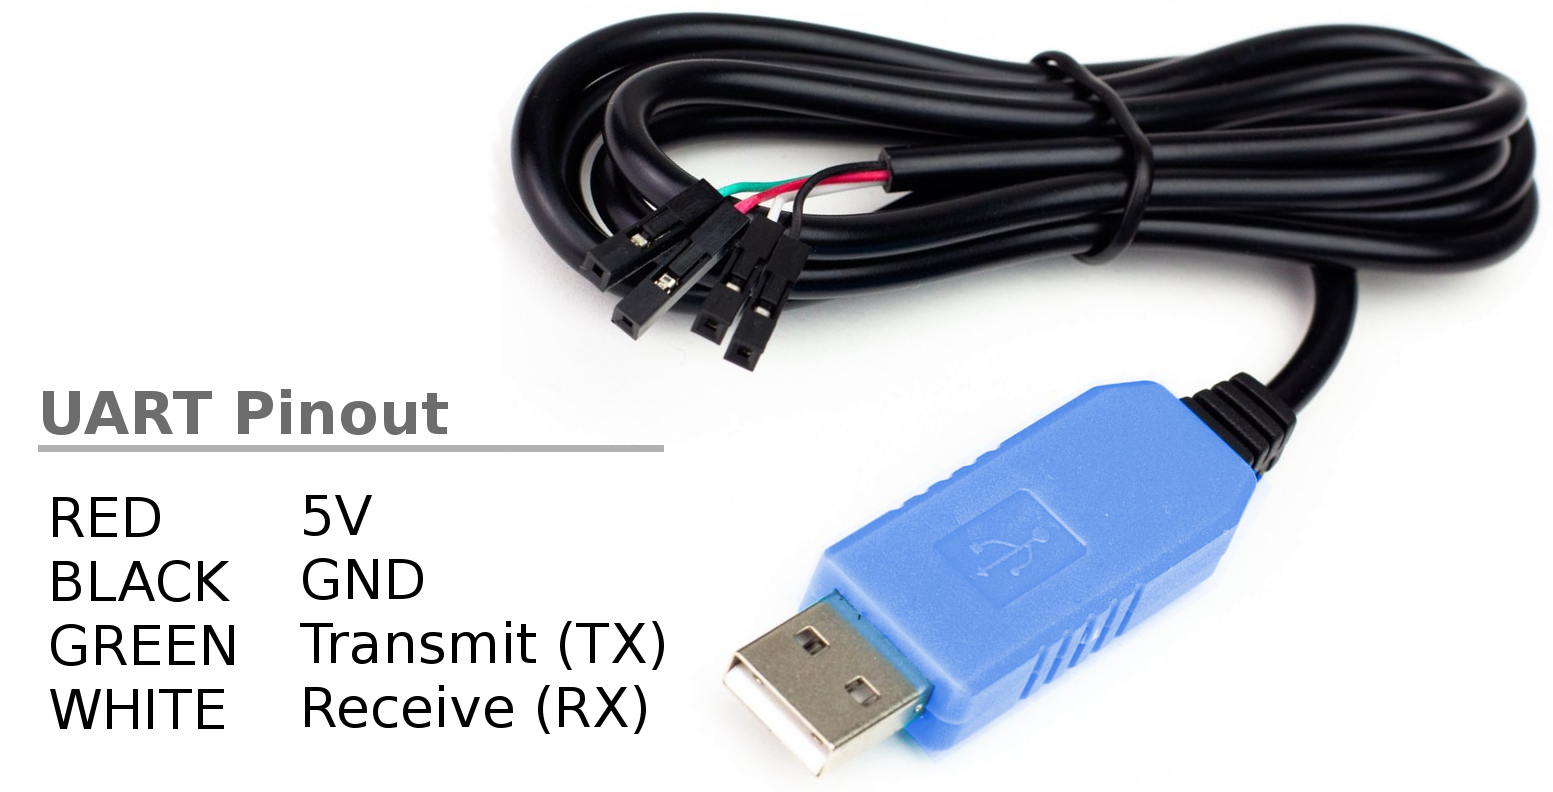
\includegraphics[width=0.6\textwidth]{usb_uart}
    \caption{Pinout of the Adafruit 954 USB-UART cable.}
    \label{usb_uart}
\end{figure}

\subsection{Finding Installed Ports on Windows}
Where to find on windows
windows calls "COM\#" located in device manager
need steps to find on lab machines.




\subsection{Using the Putty Terminal Program}
How to set up Putty

\begin{figure}[]
    \centering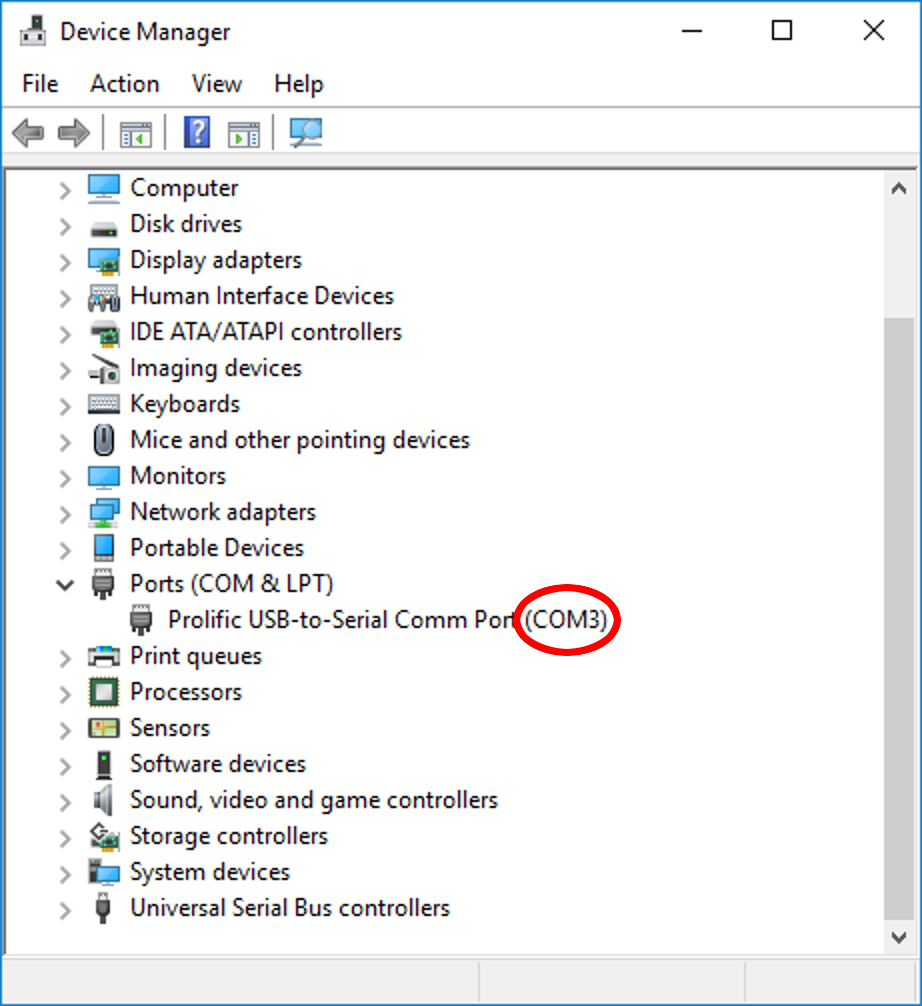
\includegraphics[height=0.45\textheight]{device_manager}
    \caption{Windows device manager with the ports tab expanded.}
    \label{device_manager}
\end{figure}
\begin{figure}[]
    \centering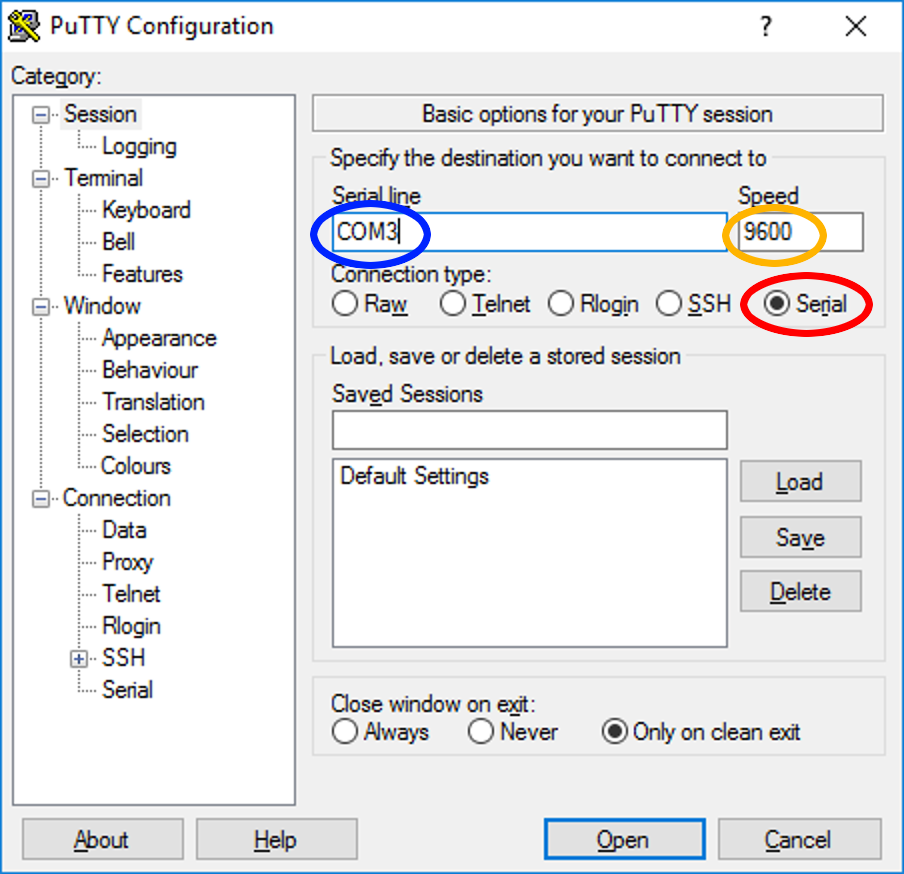
\includegraphics[height=0.40\textheight]{putty}
    \caption{Putty serial terminal}
    \label{putty}
\end{figure}
mention typing in terminal, no response
how to test cable/terminal with loopback (wire between RX/TX)

\section{Lab Assignment}
\subsection{Preparing to use the USART} 
Set up pins and connect USB-USART cable
Have them test terminal/cable with loopback
Provided code (HAL library?) to enable and test USART, should see string printed in terminal
\subsection{Blocking Transmission}	
Set up and enable USART to baud rate using registers
Transmit single char in loop to terminal
Write simple string transmit function and send strings to terminal 
mention C-strings, but tell them to look elsewhere for help with those
Capture and decode the string using the logic analyzer
include screenshot in lab report
\subsection{Blocking Reception}			
Receive single chars in loop from terminal
toggle LEDs on char match (r for red etc...)
\subsection{Interrupt-Based Reception and Command Parsing}	
Set up USART RX interrupt
set up static buffer (with basic over/underflow protection)
buffer word until newline and set flag
Use simple state machine and string match (they can write) in main program to recognize simple command strings (example: "red \\n on \\n")
Provide text feedback "ready for command", "buffer overflow", "unknown command", "invalid command", "command accepted"
\begin{figure}[]
    \centering
\includegraphics[width=\textwidth]{command_flowchart}
    \caption{Flowchart for command parsing.}
    \label{command_flowchart}
\end{figure}


\end{document}
